% Multiple Choice Question 26

\begin{center}
    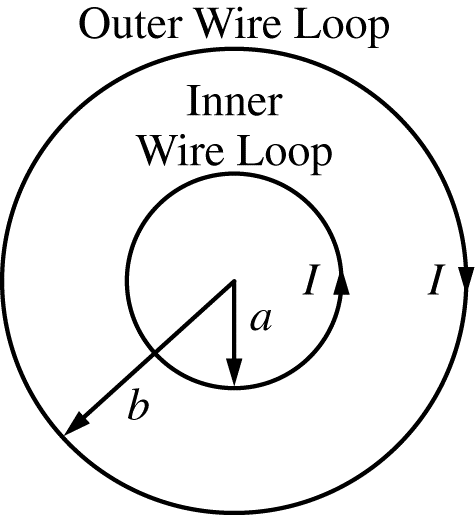
\includegraphics[scale=0.3]{images/img-013-027.png}
\end{center}

\begin{questions}\setcounter{question}{25}\question
Two concentric circular wire loops carry equal currents $I$ in opposite directions, as shown in the figure above. The inner loop has a radius $a$ and carries a counterclockwise current. The outer loop has a radius $b$ and carries a clockwise current. What is the magnitude and direction of the magnetic field at the center of the loops?

\tabto{0.75cm}\underline{Magnitude}
\tabto{4.00cm}\underline{Direction}

\begin{choices}
    \choice $\dfrac{\mu_{0} I}{2}\left(\dfrac{1}{a}-\dfrac{1}{b}\right)$    
            \tabto{3.25cm} Out of the page
    \choice $\dfrac{\mu_{0} I}{2}\left(\dfrac{1}{a}-\dfrac{1}{b}\right)$    
            \tabto{3.25cm} Into the page
    \choice Zero                                                          
            \tabto{3.25cm} Undefined since magnitude is zero  
    \choice $\dfrac{\mu_{0} I}{2 \pi}\left(\dfrac{1}{a}-\dfrac{1}{b}\right)$
            \tabto{3.25cm}  Out of the page 
    \choice $\dfrac{\mu_{0} I}{2 \pi}\left(\dfrac{1}{a}-\dfrac{1}{b}\right)$
            \tabto{3.25cm}  Into the page 
\end{choices}
\end{questions}
